%%%%%%%%%%%%%%%%%%%%%%%%%%%%%% Preamble
\documentclass[11pt]{article}
\setlength{\parskip}{\baselineskip}%
\setlength{\parindent}{0pt}%
\usepackage{amsmath,amssymb,amsthm,physics,graphicx,titling}
\newcommand{\subtitle}[1]{%
  \posttitle{%
    \par\end{center}
    \begin{center}\large#1\end{center}
    \vskip0.5em}%
}

\usepackage{graphicx}
\begin{document}

%%%%%%%%%%%%%%%%%%%%%%%%%%%%%% Heading
	\title{Ph 20 - Assignment 2}
	\author{Yovan Badal}
	\date{10/15/2017}
	\maketitle
	
%%%%%%%%%%%%%%%%%%%%%%%%%%%%%% Body
\section{Derivation of Simpson's Formula}
\subsection{Extended Formula}
We define $h_N= \frac{(b-a)}{N},and x_0=a,x_1=a+h_N,x_2=a+ 2h_N,...,x_N=b$. We then find, using Simpson's Rule, that:
\begin{align*}
\int_a^b f(x) \dd{x} &= \int_{x_0}^{x_1} f(x) \dd{x} + \int_{x_1}^{x_2} f(x) \dd{x} + ... + \int_{x_{N-1}}^{x_N} f(x) \dd{x} \\
&\approx h_N\bigg(\frac{f(x_0)}{6} + \frac{4f(\frac{x_0 + x_1}{2})}{6} + \frac{f(x_1)}{6} \bigg) \\
&+ h_N\bigg(\frac{f(x_1)}{6} + \frac{4f(\frac{x_1 + x_2}{2})}{6} + \frac{f(x_2)}{6} \bigg) \\
&+ ... + h_N\bigg(\frac{f(x_{N-1})}{6} + \frac{4f(\frac{x_{N-1} + x_N}{2})}{6} + \frac{f(x_N)}{6} \bigg) \\
&= h_N \bigg(\frac{f(x_0)}{6} + \frac{4f(\frac{x_0 + x_1}{2})}{6} + \frac{f(x_1)}{3} + \frac{4f(\frac{x_1 + x_2}{2})}{6} + \frac{f(x_2)}{3} \\
&+ ... + \frac{f(x_{N-1})}{3} + \frac{4f(\frac{x_{N-1} + x_N}{2})}{6} + \frac{f(x_N)}{6} \bigg)
\end{align*}
The last line represents the extended Simpson's Formula.
\newpage

\subsection{Local Error}
We write $f(x)$ as a Taylor sum centered at $a$:
\[
f(x) = f(a) + f'(a)(x-a) + \frac{f''(a)}{2!} (x-a)^2 + \frac{f'''(a)}{3!} (x-a)^3 + \frac{f''''(\eta)}{4!} (x-a)^4
\]
where $x, \eta \in [a,b]$ and the last term is the Lagrange remainder.

By elementary integration, we have
\[
I = f(a)H + f'(a)\frac{H^2}{2!} + f''(a)\frac{H^3}{3!} + f'''(a)\frac{H^4}{4!} + f''''(\eta)\frac{H^5}{5!}
\]

Now we find the estimate of the integral using Simpson's formula, $I_{simp}$, estimating the $f(\frac{a+b}{2})$ and $f(c)$ terms using the Taylor sum above:
\begin{align*}
I_{simp} &= H\bigg(\frac{f(a)}{6} + \frac{4}{6}\big(f(a) + f'(a)\frac{H}{2} + \frac{f''(a)}{2!} (\frac{H}{2})^2 \\
&+ \frac{f'''(a)}{3!} (\frac{H}{2})^3 + \frac{f''''(\eta)}{4!} (\frac{H}{2})^4 \big) \bigg) \\
&= f(a)H + f'(a)\frac{H^2}{2} + f''(a)\frac{H^3}{6} + f'''(a)\frac{H^4}{24} \\
&+ f''''(\eta)\frac{5H^5}{24}
\end{align*}
Therefore, we find
\[
I_{simp} - I = f''''(\eta)\frac{H^5}{5}
\]
and conclude that Simpson's Formula is locally of fifth order in H, since
\[
I = I_{simp} + O(H^5).
\]

The global error of Simpson's Formula is approximately
\[
-f''''(\xi)\frac{h_N^5}{5} = -(b-a)f''''(\xi)\frac{h_N^4}{5}
\]
where $\xi \in [a,b]$. Therefore the Extended Simpson Formula is globally of fourth order in $h_N$.
\newpage

\section{Accuracy of Numerical Integration Methods}
\subsection{Trapezoid Method - Global Error Behavior with respect to N}

\begin{figure}[htp]
\centering
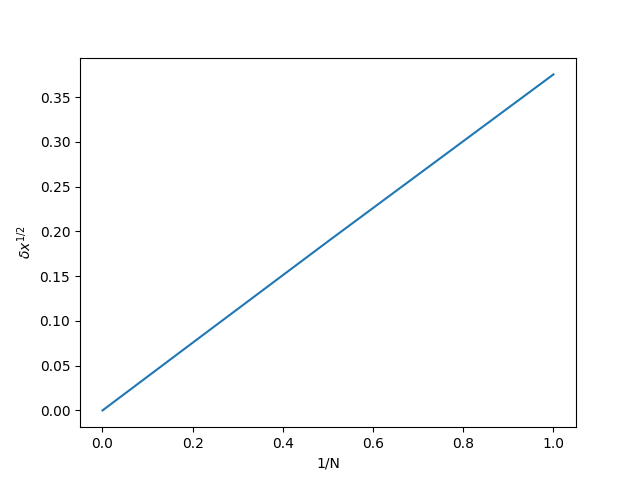
\includegraphics[scale=0.80]{trap_err_5000.png}
\caption{Error $\delta x^{\frac{1}{2}}$ plotted against 1/N.}
\label{trap_err}
\end{figure}
This plot of the square root of the global error w.r.t. $\frac{1}{N}$ clearly shows the global second order in $h_N$ behavior - the plot of $\delta x^{\frac{1}{2}}$ against $\frac{1}{N}$ is only linear if the global error $\delta x$ is $O(h_N^2)$.

\newpage

\subsection{Simpson's Method - Global Error Behavior with respect to N}

\begin{figure}[htp]
\centering
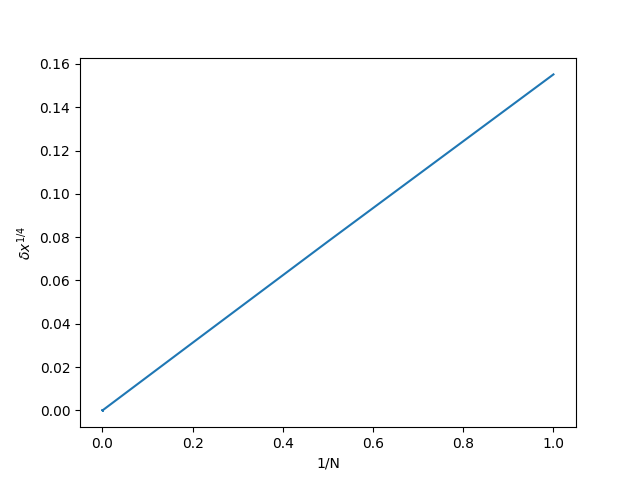
\includegraphics[scale=0.80]{simp_err_5000.png}
\caption{Error $\delta x^{\frac{1}{4}}$ plotted against 1/N.}
\label{simp_err}
\end{figure}
This plot of the square root of the global error w.r.t. $\frac{1}{N}$ clearly shows the global fourth order in $h_N$ behavior - the plot of $\delta x^{\frac{1}{4}}$ against $\frac{1}{N}$ is only linear if the global error $\delta x$ is $O(h_N^4)$.
\newpage

\subsection{Error stops decreasing for large N}
We observe that for very large N (small $\frac{1}{N}$), the global error for the Simpson method stops increasing. We observe this by taking the plot above, but for N ranging from 500 to 5000 and observing that the global error plot becomes dense.
\begin{figure}[htp]
\centering
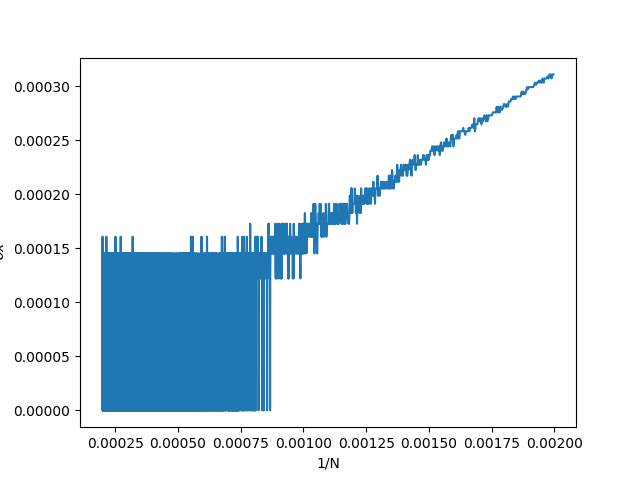
\includegraphics[scale=0.80]{simp_err_500_5000.png}
\caption{Global error for N from 500 to 5000 (Simpson's Method)}
\label{simp_dense}
\end{figure}
It is possible that at this point truncation errors become too large for higher N to increase accuracy. However, the Trapezoid method fails to stop increasing in accuracy even for higher N. This is because the Trapezoid method is less accurate to begin with, and truncation errors still do not matter even for such high N (as shown by this plot for N ranging from 40000 to 50000):
\newpage

\begin{figure}[htp]
\centering
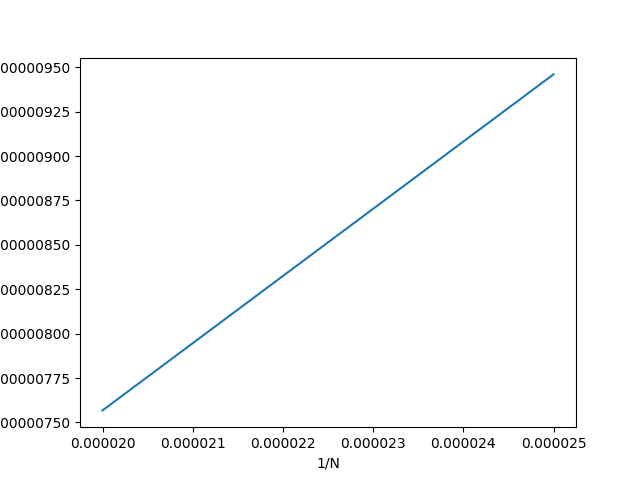
\includegraphics[scale=0.80]{trap_err_40000_50000.png}
\caption{Global error for N from 40000 to 50000 (Trapezoid Method)}
\label{trap_no_break}
\end{figure}

For even higher N, truncations will begin to matter again, but for some reason my PC freezes when I try to run the script for higher N so I have not been able to generate a dense plot for the Trapezoid error.
\newpage

\section{Other integration methods}
\subsection{Integrating $e^x$ from 0 to 1}
Expected Value = 1.71828182846 \\
Accuracy requested = 0.01 \\
Result from our routine = 1.7182818881 \\
Error = 5.96448117562e-08 \\


Scipy quad result = 1.71828182846 \\
Scipy quad error = 1.90767604875e-14 \\


Scipy Romberg result = 1.71828182846 \\
Scipy Romberg error = 3.30846461338e-14 \\

\subsection{Integrating $x^2$ from 0 to 1}
Expected Value = 0.333333333333 \\
Accuracy requested = 0.01 \\
Result from our routine = 0.333333333333 \\
Error = 0.0 \\


Scipy quad result = 0.333333333333 \\
Scipy quad error = 3.70074341542e-15 \\


Scipy Romberg result = 0.333333333333 \\
Scipy Romberg error = 0.0 \\
\end{document}